\documentclass[hyperref={pdfpagelabels=false}]{beamer}

\usepackage{lmodern,graphicx}
\usepackage{natbib}
\usepackage{pifont}
\usepackage{xcolor}
\usepackage{amsmath,amssymb}

\bibpunct[:]{(}{)}{;}{a}{}{,}
\bibliographystyle{yahapj}

\usepackage{aastex_hack}
\usepackage{tikz}
\usetikzlibrary{arrows}

\usetheme{Hannover} %OLD
%\usetheme{Copenhagen} %NEW

\usefonttheme{professionalfonts} % using non standard fonts for beamer
\usefonttheme{serif} % default family is serif
\usepackage[T1]{fontenc}
\usepackage{newtxtext,newtxmath}

\setbeamerfont{block body}{size=\tiny}

\setbeamertemplate{frametitle}[default][center]

\definecolor{myblue}{RGB}{0,0,255}
\definecolor{mypurple}{RGB}{100,0,119}
\definecolor{myred}{RGB}{200,0,0}
\definecolor{myblack}{RGB}{0,0,0}
\definecolor{mygreen}{RGB}{50,200,50}
\definecolor{myyellow}{RGB}{255,255,0}
\newcommand{\bsquare}{\item[\color{myblue}\ding{110}]}
\newcommand{\psquare}{\item[\color{mypurple}\ding{110}]}
\newcommand{\rsquare}{\item[\color{myred}\ding{110}]}
\newcommand{\blsquare}{\item[\color{myblack}\ding{110}]}
\newcommand{\gsquare}{\item[\color{mygreen}\ding{110}]}
\newcommand{\ysquare}{\item[\color{myyellow}\ding{110}]}

\title{Dark Matter in Galaxy Clusters}
\subtitle{Shape, Projection, and Environment}  
\titlegraphic{\vspace{-2.5cm}\hspace{-.8\textwidth}\includegraphics[width=.2\textwidth]{drexel-logo.png}}
\author{Austen M. Groener}
\institute[Universities]{  Drexel University }
\date{September 10, 2015}


\begin{document}

% Gets rid of 'Figure' prefix in caption
\setbeamertemplate{caption}{\raggedright\insertcaption\par}

\begin{frame}
\titlepage
\end{frame} 


%\begin{frame}
%\frametitle{Table of Contents}
%\tableofcontents
%\end{frame} 

\section{Introduction} 
\subsection{The Anatomy of a Cluster}
\begin{frame}
  \begin{figure}
    \begin{tikzpicture}
      \node[anchor=south west,inner sep=0] (image) at (0,0) {\includegraphics[width=\textwidth]{a1689.jpg}};
      \begin{scope}[x={(image.south east)},y={(image.north west)}]
        \node [anchor=west , color=white] (text1) at (0.0,0.95) {\small
          Abell 1689};
        \node [anchor=west , color=white] (text1) at (0.70,0.95) {\small
          Scale: $\sim$2 Mly};
        \node [anchor=west , color=white] (text1) at (0.70,0.90) {\small
          $z=0.183$ (2.2 Gly)};
        \node [anchor=west , color=white] (text1) at (0.0,0.15) {\small
          Credit: NASA Hubble Space Telescope};
      \end{scope}
    \end{tikzpicture}
  \end{figure}  
\end{frame}

\begin{frame}
  \begin{figure}
    \begin{tikzpicture}
      \node[anchor=south west,inner sep=0] (image) at (0,0) {\includegraphics[width=\textwidth]{a1689.jpg}};
      \begin{scope}[x={(image.south east)},y={(image.north west)}]
        \node [anchor=west , color=white] (text1) at (0.0,0.95) {\small
          Abell 1689};
        \node [anchor=west , color=white] (text1) at (0.70,0.95) {\small
          Scale: $\sim$2 Mly};
        \node [anchor=west , color=white] (text1) at (0.0,0.15) {\small
          Credit: NASA Hubble Space Telescope};
        \draw[thick, color=white] (0.605,0.44) ellipse (0.25cm and 0.25cm);
        \draw[thick,->, color=white] (0.725,0.56) -- (0.625,0.46);
        \draw[thick, color=white] (0.68,0.63) ellipse (0.3cm and 0.3cm);
        \draw[thick,->, color=white] (0.80,0.75) -- (0.705,0.655);
        \draw[thick, color=white] (0.26,0.214) ellipse (0.3cm and 0.3cm);
        \draw[thick,->, color=white] (0.14,0.334) -- (0.235,0.239);
        \draw[thick, color=white] (0.197,0.55) ellipse (0.3cm and 0.3cm);
        \draw[thick,->, color=white] (0.097,0.65) -- (0.172,0.575);
      \end{scope}
    \end{tikzpicture}
  \end{figure}  
\end{frame}


\begin{frame}
  \begin{figure}
    \begin{tikzpicture}
      \node[anchor=south west,inner sep=0] (image) at (0,0) {\includegraphics[width=\textwidth]{a1689_gas.jpg}};
      \begin{scope}[x={(image.south east)},y={(image.north west)}]
        \node [anchor=west , color=white] (text1) at (0.0,0.95) {\small
          Abell 1689};
        \node [anchor=west , color=white] (text1) at (0.70,0.95) {\small
          Scale: $\sim$2 Mly};
        \node [anchor=west , color=white] (text1) at (0.0,0.2) {\footnotesize
          Credit: X-ray: NASA/CXC/MIT/E.-H Peng et al};
        \node [anchor=west , color=white] (text1) at (0.0,0.15) {\footnotesize
          Optical: NASA/STScI};
      \end{scope}
    \end{tikzpicture}
  \end{figure}  
\end{frame}


\begin{frame}
  \begin{figure}
    \begin{tikzpicture}
      \node[anchor=south west,inner sep=0] (image) at (0,0) {\includegraphics[width=\textwidth]{a1689_gas.jpg}};
      \begin{scope}[x={(image.south east)},y={(image.north west)}]
        \node [anchor=west , color=white] (text1) at (0.0,0.95) {\small
          Abell 1689};
        \node [anchor=west , color=white] (text1) at (0.70,0.95) {\small
          Scale: $\sim$2 Mly};
        \node [anchor=west , color=white] (text1) at (0.0,0.2) {\footnotesize
          Credit: X-ray: NASA/CXC/MIT/E.-H Peng et al};
        \node [anchor=west , color=white] (text1) at (0.0,0.15) {\footnotesize
          Optical: NASA/STScI};
        \draw[thick, color=white] (0.43,0.50) ellipse (1.1cm and 1.1cm);
      \end{scope}
    \end{tikzpicture}
  \end{figure}  
\end{frame}

\begin{frame}
  \begin{figure}
    \begin{tikzpicture}
      \node[anchor=south west,inner sep=0] (image) at (0,0) {\includegraphics[width=\textwidth]{a1689.jpg}};
      \begin{scope}[x={(image.south east)},y={(image.north west)}]
        \node [anchor=west , color=white] (text1) at (0.0,0.95) {\small
          Abell 1689};
        \node [anchor=west , color=white] (text1) at (0.70,0.95) {\small
          Scale: $\sim$2 Mly};
        \node [anchor=west , color=white] (text1) at (0.0,0.15) {\small
          Credit: NASA Hubble Space Telescope};
        \draw[thick,->, color=white] (0.26,0.81) -- (0.36,0.71);
        \draw[thick,->, color=white] (0.79,0.79) -- (0.69,0.69);
        \draw[thick,->, color=white] (0.731,0.227) -- (0.631,0.327);
        \draw[thick,->, color=white] (0.143,0.272) -- (0.243,0.372);
      \end{scope}
    \end{tikzpicture}
  \end{figure}  
\end{frame}

\begin{frame}
  \begin{figure}
    \begin{tikzpicture}
      \node[anchor=south west,inner sep=0] (image) at (0,0) {\includegraphics[width=\textwidth]{a1689.jpg}};
      \begin{scope}[x={(image.south east)},y={(image.north west)}]
        \node [anchor=west , color=white] (text1) at (0.0,0.95) {\small
          Abell 1689};
        \node [anchor=west , color=white] (text1) at (0.70,0.95) {\small
          Scale: $\sim$2 Mly};
        \node [anchor=west , color=white] (text1) at (0.0,0.15) {\small
          Credit: NASA Hubble Space Telescope};
        \draw[thick,color=white] (0.19,0.73) -- (0.37,0.73) -- (0.37,0.89) --
        (0.19,0.89) -- (0.19,0.73);
      \end{scope}
    \end{tikzpicture}
  \end{figure}  
\end{frame}


\begin{frame}
  \begin{figure}
    \begin{tikzpicture}
      \node[anchor=south west,inner sep=0] (image) at (0,0)
      {\includegraphics[width=\textwidth]{a1689_zoom-1.png}};
      \begin{scope}[x={(image.south east)},y={(image.north west)}]
        \node [anchor=west , color=white] (text1) at (0.0,0.95) {\small
          Abell 1689};
        \node [anchor=west , color=white] (text1) at (0.70,0.95) {\small
          Scale: $\sim$400 kly};
        \node [anchor=west , color=white] (text1) at (0.0,0.15) {\small
          Credit: NASA Hubble Space Telescope};
        \draw[thick, color=white] (0.385,0.5) ellipse (0.3cm and 0.3cm);
        \draw[thick, color=white] (0.425,0.67) ellipse (0.3cm and 0.3cm);
        \draw[thick, color=white] (0.25,0.56) ellipse (0.3cm and 0.3cm);
        \draw[thick, color=white] (0.19,0.7) ellipse (0.3cm and 0.3cm);
      \end{scope}
    \end{tikzpicture}
  \end{figure}  
\end{frame}


\begin{frame}
  \begin{figure}
    \begin{tikzpicture}
      \node[anchor=south west,inner sep=0] (image) at (0,0) {\includegraphics[width=\textwidth]{a1689_dm.jpg}};
      \begin{scope}[x={(image.south east)},y={(image.north west)}]
        \node [anchor=west , color=white] (text1) at (0.0,0.95) {\small
          Abell 1689};
        \node [anchor=west , color=white] (text1) at (0.70,0.95) {\small
          Scale: $\sim$2 Mly};
        \node [anchor=west , color=white] (text1) at (0.0,0.15) {\footnotesize
          Credit: NASA, ESA};
      \end{scope}
    \end{tikzpicture}
  \end{figure}  
\end{frame}

\begin{frame}
  \frametitle{Hierarchical Structure Formation}
      \begin{figure}
        \includegraphics[height=0.8\textheight]{mergertree_mod.png}
        \caption{Stewart et al. (2008)}
      \end{figure}  
\end{frame}

\begin{frame}
  \frametitle{Hierarchical Structure Formation}
      \begin{figure}
        \includegraphics[height=0.9\textheight]{mergertree_mod2.png}
      \end{figure}  
\end{frame}

\subsection{The Radial Density Profile}
\begin{frame}
  \frametitle{The Navarro-Frenk-White Profile}
  \framesubtitle{NFW (1996)}
  \begin{figure}
    \begin{tikzpicture}
      \node[anchor=south west,inner sep=0] (image) at (0,0) {\includegraphics[width=\textwidth]{NFW_Cartoon_noRs.png}};
      \begin{scope}[x={(image.south east)},y={(image.north west)}]
        \node [anchor=west , color=black] (text1) at (0.40,0.85) {\small $\mathrm{\rho_{NFW} (r) = \frac{\delta_{c}\,\rho_{cr}}{\frac{r}{r_{s}} \left(1+ \frac{r}{r_{s}}\right)^{2}}}$};
      \end{scope}
    \end{tikzpicture}        
  \end{figure}
\end{frame}

\begin{frame}
  \frametitle{The Navarro-Frenk-White Profile}
  \framesubtitle{NFW (1996)}
  \begin{figure}
    \begin{tikzpicture}
      \node[anchor=south west,inner sep=0] (image) at (0,0) {\includegraphics[width=\textwidth]{NFW_Cartoon_1Rs.png}};
      \begin{scope}[x={(image.south east)},y={(image.north west)}]
        \node [anchor=west , color=black] (text1) at (0.40,0.90) {\small
          $\mathrm{\rho_{NFW} (r) =
            \frac{\delta_{c}\,\rho_{cr}}{\frac{r}{r_{s}} \left(1+
                \frac{r}{r_{s}}\right)^{2}}}$};
        \node [anchor=west , color=black] (text1) at (0.65,0.65) {\small
          1) The Scale Radius};
        \node [anchor=west , color=black] (text1) at (0.78,0.60) {\small
          $\mathrm{r_{s}}$};
        \draw[thick,->, color=black] (0.65,0.65) -- (0.53,0.55);
        \node [anchor=west , color=blue] (text1) at (0.13,0.69) {\footnotesize
          $\mathrm{\rho \propto r^{-1}}$};
        \node [anchor=west , color=blue] (text1) at (0.444,0.492) {\footnotesize
          $\mathrm{\rho \propto r^{-2}}$};
        \node [anchor=west , color=blue] (text1) at (0.73,0.22) {\footnotesize
          $\mathrm{\rho \propto r^{-3}}$};
      \end{scope}
    \end{tikzpicture}        
  \end{figure}
\end{frame}

\begin{frame}
  \frametitle{The Navarro-Frenk-White Profile}
  \framesubtitle{NFW (1996)}
  \begin{figure}
    \begin{tikzpicture}
      \node[anchor=south west,inner sep=0] (image) at (0,0) {\includegraphics[width=\textwidth]{NFW_Cartoon.png}};
      \begin{scope}[x={(image.south east)},y={(image.north west)}]
        \node [anchor=west , color=black] (text1) at (0.40,0.90) {\small
          $\mathrm{\rho_{NFW} (r) =
            \frac{\delta_{c}\,\rho_{cr}}{\frac{r}{r_{s}} \left(1+
                \frac{r}{r_{s}}\right)^{2}}}$}; 
        \node [anchor=west , color=black] (text1) at (0.53,0.65) {\small
          2) The Concentration Index};
        \node [anchor=west , color=black] (text1) at (0.68,0.59) {\small
          $\mathrm{c_{vir \equiv \frac{r_{vir}}{r_{s}}}}$};
        \node [anchor=west , color=black] (text1) at (0.68,0.52) {\footnotesize
          $\mathrm{\delta_{c} = \frac{200}{3} \frac{c^{3}}{\ln (1+c) - \frac{c}{1+c}}}$};
      \end{scope}
    \end{tikzpicture}        
  \end{figure}
\end{frame}


\begin{frame}
\frametitle{The Cuspy Halo Problem}
\framesubtitle{(The Over-Concentration Problem)}
\begin{figure}
  \begin{tikzpicture}
    \node[anchor=south west,inner sep=0] (image) at (0,0) {\includegraphics[width=\textwidth]{lowandhighconc.png}};
    \begin{scope}[x={(image.south east)},y={(image.north west)}]
      \node [anchor=west , color=black] (text1) at (0.60,0.50) {\normalsize
        Simulation}; 
      \node [anchor=west , color=black] (text1) at (0.08,0.50) {\normalsize
        Observation}; 
    \end{scope}
  \end{tikzpicture}        
\end{figure}
\begin{columns}
  \begin{column}{0.5\textwidth}
    \begin{itemize}
    \item Observed clusters: \\$\mathrm{c_{vir} = 8-12}$
    \end{itemize}
  \end{column}
  \begin{column}{0.5\textwidth}
    \begin{itemize}
    \item Simulated clusters: \\$\mathrm{c_{vir} = 4-6}$
    \end{itemize}
  \end{column}
\end{columns}
\end{frame}


\begin{frame}
  \frametitle{ The Concentration-Mass (c-M) Scaling Relation}
  \begin{columns}
    \begin{column}{0.55\textwidth}
      \begin{figure}
        \includegraphics[width=\textwidth]{Correa_CM_Relation.png}
        \caption{Simulation {\tiny (Correa et al. 2015)}}
      \end{figure}
      
    \end{column}
    \begin{column}{0.45\textwidth}
      \begin{figure}
        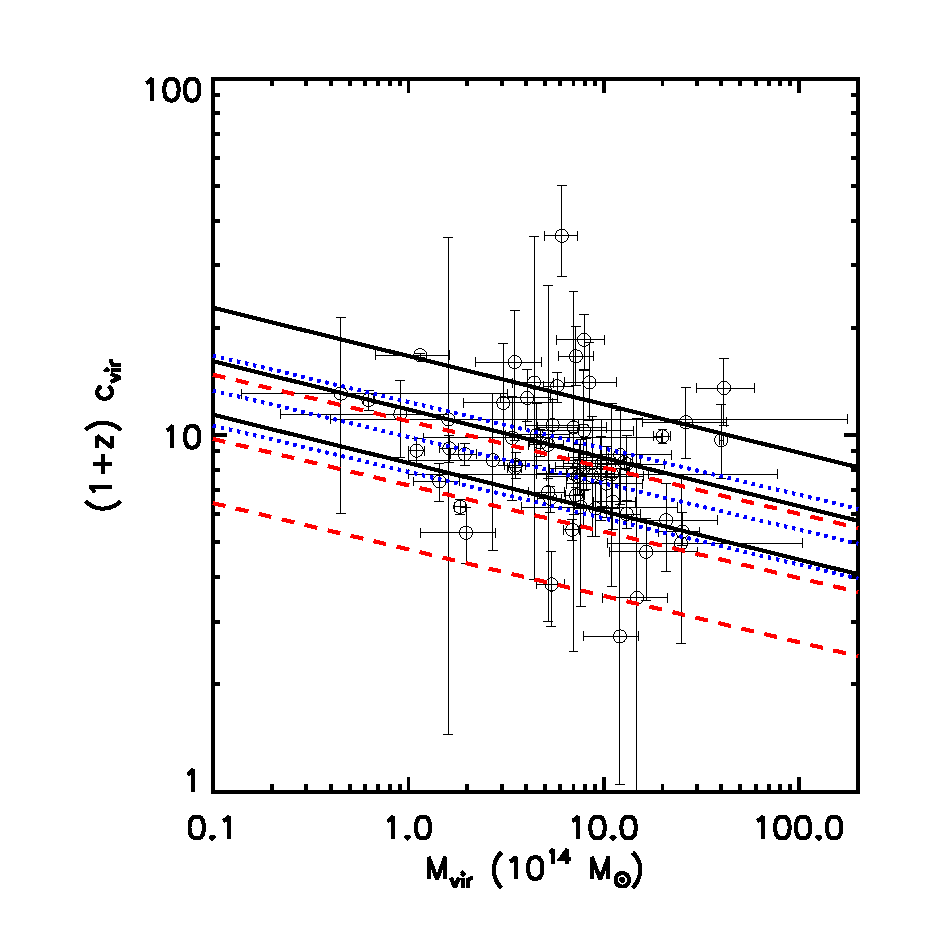
\includegraphics[width=\textwidth]{cn07.eps}
        \caption{Observational {\tiny (Comerford \& Natarajan 2007)}}
      \end{figure}
    \end{column}
  \end{columns}
\end{frame}

\subsection{Cluster Geometry}
\begin{frame}
\frametitle{Clusters Are {\em Not} Spherical}

    \centerline{Triaxial Ellipsoid}
    \begin{figure}
      \includegraphics[height=0.25\textheight]{triaxial_ellipsoid.png}
    \end{figure}  
   \begin{figure}
      \includegraphics[height=0.4\textheight]{ellipsoids2.png}
    \end{figure}  
\end{frame}

\begin{frame}
  \frametitle{Triaxial Projection Biases 2D Observables}
  \begin{figure}
    \includegraphics[width=\textwidth]{degeneracy.png}
  \end{figure}  
\end{frame}

\begin{frame}
  \frametitle{Simulated Halo Isodensities Are Not Constant On All Scales}
  \begin{figure}
    \includegraphics[width=0.7\textwidth]{hayashi.png}
    \caption{{\tiny Hayashi et al. (2007)}}
  \end{figure}  
\end{frame}

\begin{frame}
\frametitle{Implications For Cluster Mass Reconstruction}
\begin{itemize}
\item Does the changing of isodensity shape affect the concentration parameter
  {\em differently} as a function of cluster scale?
\item Is the 2D concentration even a well-defined quantity?
\end{itemize}
\end{frame}


\section{Cluster Shape \& Orientation} 
\begin{frame}
\frametitle{Groener \& Goldberg (2014)}
  \begin{columns}
    \centering
    \begin{column}{0.5\textwidth}
      \begin{block}{The MDR1 Simulation {\tiny (Prada et al. 2012)}}
        \begin{itemize}
        \item Dark matter only, $2048^{3}$ particles
        \item Adaptive-Refinement-Tree (ART) {\tiny (Kravtsov et al. 1997)}
        \item Cosmology: WMAP5
        \item Mass resolution: $\mathrm{8.721 \times 10^{9} \, M_{\odot}/h}$
        \item Force resolution: 7.0 kpc/h
        \item Box: 1000 Mpc/h (on a side)
        \item Mass range: $\mathrm{(1.7 \times 10^{11} - 1.6 \times 10^{15}) \,
            M_{\odot}/h}$
        \end{itemize}
      \end{block}
    \end{column}
    \begin{column}{0.5\textwidth}
      \begin{figure}
        \includegraphics[width=0.95\textwidth]{multidarksim.png}
      \end{figure}
    \end{column}
  \end{columns}
\end{frame}

\begin{frame}
\frametitle{MDR1 Simulated Cluster Halos}
  \begin{columns}
    \centering
    \begin{column}{0.6\textwidth}
      \begin{figure}
        \begin{tikzpicture}
          \node[anchor=south west,inner sep=0] (image) at (0,0) {\includegraphics[width=0.85\textwidth]{multidarkhalomassfunctions2.png}};
          \begin{scope}[x={(image.south east)},y={(image.north west)}]
            \draw[thick,->, color=blue] (0.65,0.8) -- (0.57,0.7);
            \node [anchor=west , color=blue] (text1) at (0.65,0.8) {\scriptsize Low};
            \draw[thick,->, color=green] (0.77,0.72) -- (0.69,0.62);
            \node [anchor=west , color=green] (text2) at (0.77,0.72) {\scriptsize Med.};
            \draw[thick,->, color=red] (0.98,0.44) -- (0.9,0.34);
            \node [anchor=west , color=red] (text3) at (0.98,0.44) {\scriptsize High};
          \end{scope}
        \end{tikzpicture}        
      \end{figure}
    \end{column}
    \begin{column}{0.4\textwidth}
      \begin{block}{\centering The Sample (z=0)}
        \begin{itemize}
        \item Low Mass: $(2.5-2.6) \times 10^{13} \mathrm{M_{\odot}/h}$ [6007]
        \item Med. Mass: $(1.0-1.1) \times 10^{14} \mathrm{M_{\odot}/h}$ [2905]
        \item High Mass: $> 1.0 \times 10^{15} \mathrm{M_{\odot}/h}$ [121]
        \end{itemize}
      \end{block}
    \end{column}
  \end{columns}
\end{frame}


\begin{frame}
\frametitle{Sample Selection Criteria}
\framesubtitle{Clustering and Virialization Criteria}
  \begin{columns}
    \centering
    \begin{column}{0.5\textwidth}
      \begin{figure}
        \includegraphics[width=\textwidth]{clustering_example.png}
        \caption{Merging, unrelaxed cluster}
      \end{figure}
      \begin{itemize}
      \item MDR1 Friends of Friends (FOF) Catalog
      \item Apply MeanShift/K-Means Algorithms
      \end{itemize}
    \end{column}
   \begin{column}{0.5\textwidth}
      \begin{figure}
        \includegraphics[width=\textwidth]{mdr1haloexample.png}
        \caption{The Final Product}
      \end{figure}
      \begin{itemize}
      \item Find Dynamically Relaxed Halos {\tiny Shaw et al. (2006)}
      \end{itemize}
    \end{column}
  \end{columns}
\end{frame}

\begin{frame}
\frametitle{Full Distribution of Shapes}
\begin{columns}
  \begin{column}{0.5\textwidth}
    \begin{figure}
      \includegraphics[width=\textwidth]{LMSingleVirialHalf.png}
    \end{figure}  
  \end{column}
  \begin{column}{0.5\textwidth}
    \begin{figure}
      \includegraphics[width=\textwidth]{pqspace_schema.png}
    \end{figure}  
  \end{column}
\end{columns}
\end{frame}


\begin{frame}
\frametitle{\centering Changing Shape of Isodensities}
\begin{block}{}
  \begin{figure}
    \begin{center}$
       \begin{array}{ccc}
        \begin{tikzpicture}
          \node[anchor=south west,inner sep=0] (image) at (0,0) {\includegraphics[scale=0.15]{p_low_1to3_half_full.pdf}};
          \begin{scope}[x={(image.south east)},y={(image.north west)}]
            \draw[ultra thick, ->, color=black] (0.3,0.75) -- (0.45,0.6);
            \node[label=below:\rotatebox{0}{\large $\mathrm{\frac{r_{200}}{2}}$}, anchor=west,color=black] at (0.2,0.925) {};
            \draw[ultra thick, ->, color=black] (0.75,0.75) -- (0.6,0.6);
            \node[label=below:\rotatebox{0}{\large $\mathrm{r_{200}}$}, anchor=west , color=black] at (0.775,0.925) {};
            \node[label=below:\rotatebox{0}{$c_{200}=1-3$}, anchor=west,color=blue] at (-0.05,0.4) {};
            \node[label=below:\rotatebox{0}{$\mathrm{p}$}, anchor=west,color=blue] at (0.82,0.45) {};
          \end{scope}
        \end{tikzpicture}        
        & \begin{tikzpicture}
          \node[anchor=south west,inner sep=0] (image) at (0,0) {\includegraphics[scale=0.15]{q_low_1to3_half_full.pdf}};
          \begin{scope}[x={(image.south east)},y={(image.north west)}]
            \node[label=below:\rotatebox{0}{$\mathrm{q}$}, anchor=west,color=blue] at (0.82,0.45) {};
          \end{scope}
        \end{tikzpicture} 
        & \begin{tikzpicture}
          \node[anchor=south west,inner sep=0] (image) at (0,0) {\includegraphics[scale=0.15]{pq_low_1to3_half_full_diff.pdf}};
          \begin{scope}[x={(image.south east)},y={(image.north west)}]
            \draw[thick] (0.625,0.45) ellipse (0.35cm and 0.7cm);
            \node[label=below:\rotatebox{0}{\footnotesize $\mathrm{\Delta p = 0.14}$}, anchor=west , color=black] at (0.225,0.825) {};
            \node[label=below:\rotatebox{0}{\footnotesize $\mathrm{\Delta q = 0.11}$}, anchor=west , color=black] at (0.225,0.6) {};
          \end{scope}
        \end{tikzpicture} \\
        \begin{tikzpicture}
          \node[anchor=south west,inner sep=0] (image) at (0,0) {\includegraphics[scale=0.15]{p_low_7to10_half_full.pdf}};
          \begin{scope}[x={(image.south east)},y={(image.north west)}]
            \node[label=below:\rotatebox{0}{$c_{200}=7-10$}, anchor=west,color=blue] at (-0.03,0.4) {};
            \node[label=below:\rotatebox{0}{$\mathrm{p}$}, anchor=west,color=blue] at (0.82,0.875) {};
          \end{scope}
        \end{tikzpicture}        
        & \begin{tikzpicture}
          \node[anchor=south west,inner sep=0] (image) at (0,0) {\includegraphics[scale=0.15]{q_low_7to10_half_full.pdf}};
          \begin{scope}[x={(image.south east)},y={(image.north west)}]
            \node[label=below:\rotatebox{0}{$\mathrm{q}$}, anchor=west,color=blue] at (0.82,0.875) {};
          \end{scope}
        \end{tikzpicture} 
        & \begin{tikzpicture}
          \node[anchor=south west,inner sep=0] (image) at (0,0) {\includegraphics[scale=0.15]{pq_low_7to10_half_full_diff.pdf}};
          \begin{scope}[x={(image.south east)},y={(image.north west)}]
            \draw[thick] (0.575,0.45) ellipse (0.25cm and 0.7cm);
            \node[label=below:\rotatebox{0}{\footnotesize $\mathrm{\Delta p = 0.03}$}, anchor=west , color=black] at (0.225,0.825) {};
            \node[label=below:\rotatebox{0}{\footnotesize $\mathrm{\Delta q = 0.03}$}, anchor=west , color=black] at (0.225,0.6) {};
          \end{scope}
        \end{tikzpicture}
        \end{array}$
      \end{center}
      \caption{\tiny{{\em Along the Top}: Distribution of axial ratios p, q,
      on characteristic scales $r_{200}/2$ (blue), and $r_{200}$
      (green) for $c_{200}=1-3$. Difference in axial ratios p (purple) and q (orange) on
      these scales. {\em Along the Bottom}: Similar plots for $c_{200}=7-10$.}}
    \end{figure}
  \end{block}
\end{frame}

\begin{frame}
\frametitle{\centering Concentrations In Projection}
\begin{block}{}
  \begin{figure}
    \begin{center}$
       \begin{array}{cc}
        \begin{tikzpicture}
          \node[anchor=south west,inner sep=0] (image) at (0,0) {\includegraphics[width=0.5\textwidth]{LMSingleVirialHalfConcsLOS2.jpg}};
          \begin{scope}[x={(image.south east)},y={(image.north west)}]
            \draw[ultra thick, color=red] (0.308,0.525) -- (0.779,0.273);
            \node [anchor=west , color=black] (text1) at (0.5,1.02) {\small
              r200/2};
          \end{scope}
        \end{tikzpicture}        
        & \begin{tikzpicture}
          \node[anchor=south west,inner sep=0] (image) at (0,0) {\includegraphics[width=0.5\textwidth]{LMSingleVirialFullConcsLOS2.jpg}};
          \begin{scope}[x={(image.south east)},y={(image.north west)}]
            \draw[ultra thick, color=red] (0.305,0.39) -- (0.779,0.257);
            \node [anchor=west , color=black] (text1) at (0.5,1.0) {\small
              r200};
          \end{scope}
        \end{tikzpicture} 
        \end{array}$
      \end{center}
    \end{figure}
  \end{block}
  \begin{itemize}
  \item Trend 1: Projected concentration is a function of
    intrinsic concentration, and is fractionally larger for low
    concentrations.
  \end{itemize}
\end{frame}

\begin{frame}
\frametitle{\centering Concentrations In Projection}
\begin{block}{}
  \begin{figure}
    \begin{center}$
      \begin{array}{cc}
        \begin{tikzpicture}
          \node[anchor=south west,inner sep=0] (image) at (0,0) {\includegraphics[width=0.5\textwidth]{LMSingleVirialHalfConcsLOS2.jpg}};
          \begin{scope}[x={(image.south east)},y={(image.north west)}]
            \draw[ultra thick, color=red] (0.308,0.525) -- (0.779,0.273);
            \node [anchor=west , color=black] (text1) at (0.5,1.02) {\small
              r200/2};
          \end{scope}
        \end{tikzpicture}        
        & \begin{tikzpicture}
          \node[anchor=south west,inner sep=0] (image) at (0,0) {\includegraphics[width=0.5\textwidth]{LMSingleVirialFullConcsLOS2.jpg}};
          \begin{scope}[x={(image.south east)},y={(image.north west)}]
            \draw[ultra thick, color=red] (0.308,0.525) -- (0.779,0.273);
            \draw[ultra thick, color=blue] (0.305,0.39) -- (0.779,0.257);
            \draw[thick, ->, color=black] (0.2,0.7) -- (0.2,0.55);
            \draw[thick, color=black] (0.15,0.525) -- (0.25,0.525);
            \draw[thick, ->, color=black] (0.2,0.25) -- (0.2,0.375);
            \draw[thick, color=black] (0.15,0.4) -- (0.25,0.4);
            \node[label=below:\rotatebox{0}{\footnotesize $\mathrm{\sim 18
                \%}$}, anchor=west , color=black] at (0.425,0.75) {};
            \node [anchor=west , color=black] (text1) at (0.5,1.0) {\small
              r200};
          \end{scope}
        \end{tikzpicture} 
        \end{array}$
      \end{center}
    \end{figure}
  \end{block}
  \begin{itemize}
  \item Trend 2: Projected concentration is a function of radius,
    and changes the most for intrinsically low concentrations.
  \end{itemize}
\end{frame}

\begin{frame}
\frametitle{Conclusions}
\begin{block}{}
\begin{itemize}
\item {\large Relaxed MDR1 cluster halos are prolate spheroidal in shape,
  and move toward sphericity at larger radii.}
\item {\large Due to analytical projection, line-of-sight oriented halos are
  over-concentrated.}
\item {\large This over-concentration is stronger on SL scales than on WL scales
  ($\mathrm{\sim 20\%}$).}
\item {\large Lower mass halos {\scriptsize ($\mathrm{\sim 3 \times 10^{13}
        \,h^{-1} M_{\odot}}$)} are {\em more} affected by this difference than 
    high mass halos are.} 
\end{itemize}
\end{block}

\begin{figure}
  \begin{tikzpicture}
    \node[anchor=south west,inner sep=0] (image) at (0,0)
    {\includegraphics[width=\textwidth]{paper1.png}};
    \node[inner sep=0pt] (whitehead) at (0.22,0.9)
    {\includegraphics[width=.10\textwidth]{qrcode.png}};
  \end{tikzpicture}
\end{figure}
\end{frame}

\begin{frame}
\frametitle{The c-M Relation: What To Expect}
\begin{figure}
\centering
\includegraphics[width=0.75\textwidth]{cM_expect.png}
\end{figure}
\end{frame}



\section{The Observed c-M Relation} 

\begin{frame}
  \frametitle{Groener, Goldberg, \& Sereno (2015)}
  \begin{columns}
    \centering
    \begin{column}{0.5\textwidth}
      \begin{itemize}
      \item {\footnotesize 81 papers}
      \item {\footnotesize 781 cluster measurements}
      \item {\footnotesize 361 unique clusters}
      \item Methods: \\
        {\tiny (arranged roughly from small to large scale)}
        \begin{itemize}
          \gsquare{\footnotesize X-ray}
          \rsquare{\footnotesize Strong Lensing (SL)}
          \blsquare{\footnotesize Weak + Strong Lensing (WL+SL)}
          \psquare{\footnotesize Weak Lensing (WL)}
          \ysquare{\footnotesize Line of sight velocity dispersion (LOSVD)} 
          \bsquare{\footnotesize Caustic Method (CM)}
        \end{itemize}
      \end{itemize}
    \end{column}
    \begin{column}{0.5\textwidth}
      \begin{figure}
        \includegraphics[width=\textwidth]{CMRelation_FullSample_Symmetrized.png}
      \end{figure}
    \end{column}
  \end{columns}
\end{frame}

\begin{frame}
  \frametitle{Lensing Reconstruction Techniques}
  \framesubtitle{Weak Lensing (WL), Strong Lensing (SL), and WL+SL}
  \begin{columns}
    \begin{column}{0.45\textwidth}
      \begin{block}{}
        \begin{figure}
          \begin{tikzpicture}
            \node[anchor=south west,inner sep=0] (image) at (0,0) {\includegraphics[width=\textwidth]{oguri.png}};
            \begin{scope}[x={(image.south east)},y={(image.north west)}]
              \draw[thick,color=black] (0.49,0.43) -- (0.65,0.43) -- (0.65,0.62) --
              (0.49,0.62) -- (0.49,0.43);
            \end{scope}
          \end{tikzpicture}
          \caption{Abell 2390 (z=0.228) {\tiny Oguri et al. (2010)}}
        \end{figure}  
      \end{block}
    \end{column}
    \begin{column}{0.55\textwidth}
      \begin{block}{}
        \begin{figure}
          \includegraphics[width=\textwidth]{jauzac.pdf}
          \caption{Abell 2744 (z=0.308) {\tiny Jauzac et al. (2014)}}
        \end{figure}
      \end{block}
    \end{column}
  \end{columns}
\end{frame}

\begin{frame}
\frametitle{Galaxy-Based Reconstruction Techniques}
\framesubtitle{The Caustic Method (CM) and Line-of-sight Velocity Dispersion
  (LOSVD)}
      \begin{figure}
        \includegraphics[width=0.9\textwidth]{rines.png}
        \caption{The Caustic Method {\tiny Rines et al. (2006)}}
      \end{figure}
\end{frame}

\begin{frame}
\frametitle{X-ray Reconstruction Techniques}
  \begin{figure}
    \begin{tikzpicture}
      \node[anchor=south west,inner sep=0] (image) at (0,0) {\includegraphics[height=0.9\textheight]{a1689_gas.jpg}};
      \begin{scope}[x={(image.south east)},y={(image.north west)}]
        \node [anchor=west , color=white] (text1) at (0.0,0.95) {\small
          Abell 1689};
        \node [anchor=west , color=white] (text1) at (0.70,0.95) {\small
          Scale: $\sim$2 Mly};
        \node [anchor=west , color=white] (text1) at (0.0,0.1) {\footnotesize
          Credit: X-ray: NASA/CXC/MIT/E.-H Peng et al};
        \node [anchor=west , color=white] (text1) at (0.0,0.05) {\footnotesize
          Optical: NASA/STScI};
      \end{scope}
    \end{tikzpicture}
  \end{figure}  
\end{frame}

\begin{frame}
\frametitle{Reconstruction-Dependent Results}
  \begin{figure}
    \includegraphics[width=\textwidth]{FitToEachMethod_Mod.png}
  \end{figure}  
\end{frame}

\begin{frame}
  \frametitle{Comparison of c-M relations}
  \begin{figure}
    \includegraphics[width=\textwidth]{fit_comparison2.png}
  \end{figure}  
\end{frame}

\begin{frame}
\frametitle{Fit To All Data}
  \begin{columns}
    \begin{column}{0.5\textwidth}
      \begin{figure}
        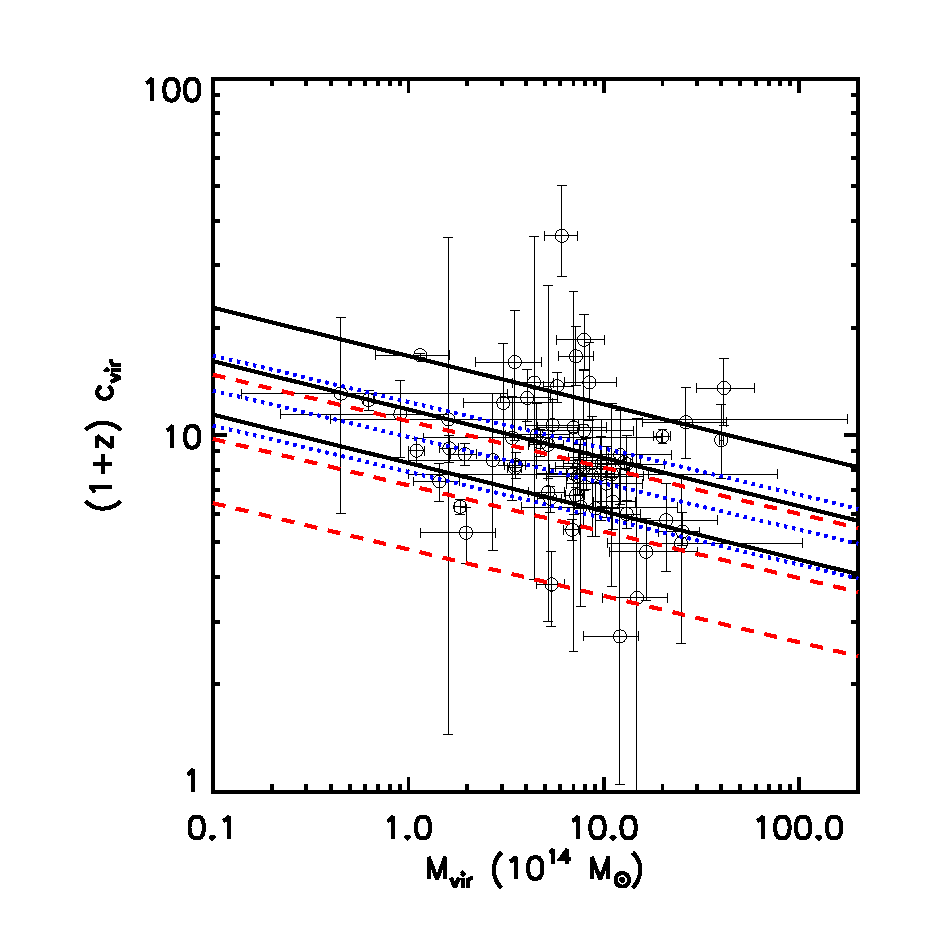
\includegraphics[width=\textwidth]{cn07.eps}
        \caption{Comerford \& Natarajan (2007) - All Methods.}
      \end{figure}  
    \end{column}
    \begin{column}{0.5\textwidth}
      \begin{figure}
        \includegraphics[width=\textwidth]{AllMethodsWithSims_linearmodel_witherror.png}
        \caption{This work - All Methods.}
      \end{figure}
    \end{column}
  \end{columns}
\end{frame}

\begin{frame}
  \frametitle{Comparison Revisited}
  \begin{figure}
    \includegraphics[width=\textwidth]{fit_comparison.png}
  \end{figure}

\centerline{Information about the halo is lost!}

\end{frame}


\begin{frame}
\frametitle{Comparison With CLASH}
\framesubtitle{Merten et al. (2014)}
  \begin{columns}
    \centering
    \begin{column}{0.5\textwidth}
      \begin{figure}
        \includegraphics[width=\textwidth]{Clash_Comparison_05.png}
        \caption{$z=0.5$}
      \end{figure}
    \end{column}
    \begin{column}{0.5\textwidth}
      \begin{figure}
        \includegraphics[width=\textwidth]{Clash_Comparison_02.png}
        \caption{$z=0.2$}
      \end{figure}
    \end{column}
  \end{columns}
    \begin{itemize}
    \item Low redshift cluster concentrations are off by $\mathrm{\sim 50\%}$
      for WL, but $\mathrm{\sim 100\%}$ for WL+SL.
    \item High redshift cluster concentrations are nearly in agreement with WL,
      but still off by $\mathrm{\sim 50\%}$ with WL+SL.
    \end{itemize}
\end{frame}

\begin{frame}
  \frametitle{Comparison With Simulations}
  \begin{columns}
    \centering
    \begin{column}{0.5\textwidth}
      \begin{figure}
        \begin{tikzpicture}
          \node[anchor=south west,inner sep=0] (image) at (0,0) {\includegraphics[width=\textwidth]{SimsComparison1.png}};
          \begin{scope}[x={(image.south east)},y={(image.north west)}]
            \node [anchor=west , color=black] (text1) at (0.24,0.95) {\small
              Recent Simulations};
          \end{scope}
        \end{tikzpicture}
      \end{figure}  
    \end{column}
    \begin{column}{0.5\textwidth}
      \begin{figure}
        \begin{tikzpicture}
          \node[anchor=south west,inner sep=0] (image) at (0,0) {\includegraphics[width=\textwidth]{SimsComparison2.png}};
          \begin{scope}[x={(image.south east)},y={(image.north west)}]
            \node [anchor=west , color=black] (text1) at (0.09,0.95) {\small
              L.O.S. Projected Sims (q=0.5)};
          \end{scope}
        \end{tikzpicture}
      \end{figure}  
    \end{column}
  \end{columns}
  \begin{itemize}
  \item Projection is not enough. Still off by almost a factor of 2!
  \item Selection effects are likely responsible.
  \end{itemize}
\end{frame}

\begin{frame}
\frametitle{Conclusions}
\begin{block}{}
\begin{itemize}
\item {\large The c-M relation varies from technique to technique.}
\item {\large The steepest relations are WL and WL+SL.}
\item {\large The WL+SL relation is steeper (though consistent) with WL.}
\item {\large The SL, CM, and LOSVD relations are not well-constrained, and
    are consistent with a slope of zero.}
\end{itemize}
\end{block}
\centerline{Look for us in MNRAS!}
\end{frame}

\section{Clusters and the LSS of the Universe}

\begin{frame}
\frametitle{The Large-Scale Cluster Environment}
  \begin{figure}
    \begin{tikzpicture}
      \node[anchor=south west,inner sep=0] (image) at (0,0) {\includegraphics[width=0.9\textwidth]{seqF_063a_half.jpg}};
      \begin{scope}[x={(image.south east)},y={(image.north west)}]
        \draw[thick,->, color=white] (0.25,0.69) -- (0.425,0.54);
        \draw[thick,->, color=white] (0.30,0.20) -- (0.45,0.45);
        \draw[thick,->, color=white] (0.80,0.43) -- (0.55,0.505);
        \node [anchor=west , color=white] (text1) at (0.0,0.07) {\scriptsize
          Bolshoi Simulation {\tiny (Klypin et al. 2011)}};
      \end{scope}
    \end{tikzpicture}
  \end{figure}  
\end{frame}

\begin{frame}
  \frametitle{The SDSS DR10 Sample}
  \begin{figure}
    \includegraphics[width=0.75\textwidth]{sdss_data_trim.png}
  \end{figure}  
  
  \begin{itemize}
  \item $\sim 1.4$ million spectroscopically confirmed galaxies
  \item $\mathrm{z \lesssim0.7}$.
  \item 203 of 361 clusters are within the survey volume.
  \end{itemize}

\end{frame}

\begin{frame}
\frametitle{Clusters Within the LSS}
    \begin{figure}
      \includegraphics[width=\textwidth]{sample_slice.png}
    \end{figure}
\end{frame}

\begin{frame}
  \frametitle{Selecting SDSS Galaxies Around Clusters}
  \begin{figure}
    \includegraphics[width=0.75\textwidth]{Abell1238.png}
  \end{figure}
\end{frame}

\begin{frame}
  \frametitle{Cluster Concentration - LSS Orientation Correlation}
  \begin{figure}
    \includegraphics[width=0.7\textwidth]{Conc_Corr2.png}
  \end{figure}
  \begin{itemize}
  \item No correlation between LSS orientation and mass and concentration.
  \item Techniques: WL (5), X-ray (33), CM (62), and LOSVD (34).
  \end{itemize}
\end{frame}

\begin{frame}
\frametitle{Future Work}
\begin{itemize}
\item Explore alternate ways of quantifying the directionality of LSS around clusters.
\item More data - particularly lensing measurements.
\item Correct for redshift space distortions like Finger of God Effect, and the
  Kaiser Effect, which may alter the distribution of galaxies (e.g. - use
  cluster membership catalogs like maxBCG).
\end{itemize}
\end{frame}

\section{Conclusions}
\begin{frame}
\frametitle{Conclusions}
{\footnotesize
    \begin{itemize}
    \item Cluster halos are prolate spheroidal on small scales, and become
      spherical on larger scales.
    \item The changing of shape alters the 2D concentration on WL and SL scales
      differently. 
    \item Low-mass clusters are affected by this difference the most.
    \end{itemize}
}

    \begin{center}
      \line(1,0){450}
    \end{center}
{\footnotesize
    \begin{itemize}
    \item The c-M relation for clusters varies significantly from technique-to-technique.
    \item WL and WL+SL are the steepest relations.
    \item WL and WL+SL are inconsistent with theory, even after projection
      effects are taken into account. This likely points to selection effects
      as the cause.
    \end{itemize}
}

    \begin{center}
      \line(1,0){450}
    \end{center}
{\footnotesize
    \begin{itemize}
    \item Cluster concentrations and masses show no correlation with the line-of-sight
      orientation of large scale structure (scales of $\mathrm{10\,h^{-1}Mpc}$).
    \end{itemize}
}
\end{frame}

\begin{frame}
\centerline{Thank you!}
\begin{itemize}
\item Advisor: Dr. David Goldberg
\item Collaborator: Dr. Mauro Sereno
\item Committee: Dr. Michael Vogeley, Dr. Gordon Richards, Dr. Luis Cruz, Dr. Andrew Hicks
\item Research Group (Current and Past): Justin Bird and Markus Rexroth
\item My Friends and Family
\item This work was also supported by the NSF (Grant 0908307).
\end{itemize}
\begin{figure}
\centering
\includegraphics[height=0.20\textheight]{NSF_logo.jpg}
\end{figure}
\end{frame}


\appendix

%\begin{frame}[allowframebreaks]
%  \bibliography{allrefs}
%\end{frame}

\begin{frame}
\frametitle{The Connection Between $\mathrm{c_{vir}}$ and $\mathrm{M_{vir}}$}
        \begin{itemize}
        \item Low-mass halos form halos earlier than massive ones
        \item The core density (concentration) of the halo reflects the density of the universe
          at the formation time
        \item Since the density of the universe decreases with time, low-mass
          halos tend to have higher concentrations 
        \end{itemize}
\end{frame}

\begin{frame}
 Shape and Density profiles are obtained for all clusters which meet
 our selection criteria.
      \begin{block}{\centering Density Profiles}
       Iterative, Moment of Inertia Tensor
       \[ \scalebox{1.4}{$\mathrm{I_{ij} = \sum w_{g}(\zeta) m_{p} (r_{i,n} -
       \bar{r_{i}}) (r_{j,n} - \bar{r_{j}})}$} \]
       Gaussian weighting function $\mathrm{w_{g} (\zeta)}$, which matches
       shape and orientation at each step
      \end{block}
      \begin{block}{\centering Model Fitting}
        Using Maximum-Likelihood Methods, we fit the NFW profile to
        halo density profiles obtained through our analysis
        \[ \scalebox{1.4}{$\mathrm{\rho_{NFW} (r) =
        \frac{\delta_{c_{200}}\rho_{cr}}{\frac{r}{r_{s}} \left(1+ \frac{r}{r_{s}}\right)^{2}}}$} \]
      \end{block}
\end{frame}

\begin{frame}
\frametitle{Cluster Timescales}
\begin{itemize}
\item {\tiny Two-Body Relaxation:
\[ t_{relax} = 2\times 10^{10} \left( \frac{V_{r}}{1000\,km/s} \right) \left(
  \frac{M_{g}}{10^{12} M_{\odot}} \right)^{-2} \left(
  \frac{N_{d}}{1000\,gal/Mpc^{3}} \right)^{-1}\]
$V_{r}$ is the radial component of the 3D velocity dispersion ($\approx 1000
km/s$), $M_{g}$ is the mass of the galaxy (or particle), and $N_{d}$ is the
number of galaxies (or particles) per $Mpc^{3}$.}
\item {\tiny Cooling Timescale: 
\[ \tau_{cool} = 9\times 10^{7} \left( T_{8} \right)^{1/2} \left( n_{e}
\right)^{-1} \,years\]
$T_{8}$ is the temerature in units of $10^{8}K$, and $n_{e}$ is measured in
particles per $cm^{-3}$ (typically $n_{e} \le 10^{-3}$)}.
\item {\tiny Dynamical Timescale:
\[ \tau_{dyn} = 6\times10^{11} \left( \frac{R}{Mpc}\right) \left(
  \frac{V_{r}}{1000\,km/s} \right) \, years \] }
\end{itemize}
\end{frame}

\begin{frame}
  \frametitle{Modeling The Observed c-M Relations}
  \begin{columns}
    \begin{column}{0.5\textwidth}
      \begin{block}{Power-Law Model}
        \begin{itemize}
        \item $\mathrm{c_{vir} = \frac{A}{1+z} \left( \frac{M_{vir}}{M_{*}}
          \right)^{\alpha}}$
        \item Constant: $\mathrm{M_{*}}$
        \item Free parameters: A, $\mathrm{\alpha}$ 
        \end{itemize}
      \end{block}
    \end{column}
    \begin{column}{0.5\textwidth}
      \begin{block}{Linear Model}
        \begin{itemize}
        \item $\mathrm{\mathcal{Y} = m\mathcal{X}+b + \epsilon}$   
        \item $\mathrm{\mathcal{Y} \equiv \log c (1+z)}$
        \item $\mathrm{\mathcal{X} \equiv \log M}$
        \item $\mathrm{m = \alpha}$
        \item $\mathrm{b = \log A - \alpha \log M_{*}}$
        \item $\mathrm{\epsilon \sim \mathcal{N}(0,\sigma_{int})}$
        \end{itemize}
      \end{block}
    \end{column}
  \end{columns}
\end{frame}

\begin{frame}
\frametitle{Measurement Uncertainty}
\framesubtitle{...and other considerations.}
\begin{itemize}
\item Arbitrary propagation of uncertainty (assuming errors are not
  independent):
\[ \delta q  \leq \left| \frac{\partial q}{\partial x} \right| + \ldots + \left|
  \frac{\partial q}{\partial z} \right| \]
This applies when we fit the c-M relation as a linear model (instead of the
original power-law model). We also apply this for re-calculating the
uncertainties for $\mathrm{c(1+z)}$ (e.g. - $q = Bx$; $\delta q = |B|\delta
x$).
\item Best-fit values and confidence intervals to expectation values and
  standard deviations (D'Agostini 2004). Starting with
  ${\theta_m}^{\Delta_{+}}_{\Delta _{-}}$. 
\[ \sigma_{\theta} \approx \frac{\Delta_{+} + \Delta_{-}}{2} \]
\[ E[\theta] \approx \theta_{m} + \mathcal{O}(\Delta_{+} -\Delta_{-}) \]
\end{itemize}
\end{frame}

\begin{frame}
\frametitle{Measurement Uncertainty}
\framesubtitle{...and other considerations.}
\begin{itemize}
\item Concentation Convention: Renormalize the concentration (and mass) based
  upon a different definition of $\mathrm{r_{vir}}$ (see procedure along with
  fitting formulae from Hu \& Kravtsov 2002).
\item Correct for cosmology: We develop our own cosmology correction. This
  turns out to be a rather small correction (of order a few percent), unless
  cosmology is extremely different from the assumed fiducial cosmology
  $\Omega_{m} = 0.3$, $\Omega_{\Lambda} = 0.7$.
\end{itemize}
\end{frame}

\begin{frame}
\frametitle{Quantifying The Angular Distribution}
\begin{block}{\centering Spherical Harmonics}
  \begin{itemize}
  \item Series: $\mathrm{f(\theta,\phi) = \sum_{l=0}^{\infty} \sum_{m=0}^{l} A_{l}^{m}
      Y_{l}^{m} (\theta,\phi)}$
  \item $\mathrm{A_{l}^{m} = \frac{4\pi}{N} \sum_{i=1}^{N_{gal}} \tilde{Y_{l}^{m}}(\theta_{i},\phi_{i})}$
  \end{itemize}
  \begin{subequations}
    \begin{equation*}
      \mathrm{Y_{1}^{1} = -\sqrt{\frac{3}{8\pi}} \sin \theta \,e^{i\phi}}
    \end{equation*}    
    \begin{equation*}
      \mathrm{Y_{1}^{0} = \sqrt{\frac{3}{4\pi}} \cos \theta}
    \end{equation*}
   \begin{equation*}
      \mathrm{Y_{1}^{-1} = \sqrt{\frac{3}{8\pi}} \sin \theta \,e^{-i\phi}}
    \end{equation*}
 \end{subequations}
 \begin{itemize}
 \item Compute for each cluster: $\mathrm{\frac{A_{1}^{0}}{\sqrt{{A_{1}^{0}}^{2}+{A_{1}^{0}}^{2}}}}$
 \item $\mathrm{A_{1}^{0}}$ tells us about line-of-sight direction.
 \end{itemize}
\end{block}
\end{frame}




\end{document}
